% \documentclass[11pt]{article}
% \usepackage[utf8]{inputenc}	% Para caracteres en español
% \usepackage{amsmath,amsthm,amsfonts,amssymb,amscd}
% \usepackage{multirow,booktabs}
% \usepackage[table]{xcolor}
% \usepackage{fullpage}
% \usepackage{lastpage}
% \usepackage{enumitem}
% \usepackage{fancyhdr}
% \usepackage{mathrsfs}
% \usepackage{wrapfig}
% \usepackage{setspace}
% \usepackage{calc}
% \usepackage{multicol}
% \usepackage{cancel}
% \usepackage[retainorgcmds]{IEEEtrantools}
% \usepackage[margin=3cm]{geometry}
% \usepackage{amsmath}
% \newlength{\tabcont}
% \setlength{\parindent}{0.0in}
% \setlength{\parskip}{0.05in}
% \usepackage{empheq}
% \usepackage{framed}
% \usepackage[most]{tcolorbox}
% \usepackage{xcolor}
% \colorlet{shadecolor}{orange!15}
% \geometry{margin=1in, headsep=0.25in}

\documentclass[11pt]{article}
 
\usepackage[margin=1in]{geometry} 
\usepackage{amsmath,amsthm,amssymb,scrextend}
\usepackage{fancyhdr}
\usepackage{graphicx}
\setlength{\headheight}{14pt}
\usepackage{xcolor}
\usepackage{color,soul}
\usepackage{gensymb}
\pagestyle{fancy}


\begin{document}
 
% --------------------------------------------------------------
%                         Start here
% --------------------------------------------------------------

\lhead{EE267 Virtual Reality}
\chead{Homework 6 Answers}
\rhead{Bohan Li}

\section{Theoretical Part}
\subsection{Rotation Quaternions}



The rotation quaternion with the rotation angle as $\theta$ and rotation axis $\textbf{v} = (v_x, v_y, v_z)^T $ is given as:
\begin{align}
    q(\theta,v) = \cos(\theta/2) + i v_x \sin(\theta/2) + j v_y \sin(\theta/2) + k v_z \sin(\theta/2).
\end{align}
The length of $q$ is \[|q| = \sqrt{\cos^2(\theta/2)+( v_x^2 + v_y^2 + v_z^2) \sin^2(\theta/2)} = \cos^2(\theta/2) + \sin^2(\theta/2) = 1.\]

\subsection{3-D Gyro Integration}
\subsubsection*{(i)}
The refresh rate is $1\ Hz$ so the time step is given as $1\ s$. The angle of rotation is given as $||\omega||\Delta{t}$ and the rotation axis is $\frac{\omega}{||\omega||}$. Therefore, the rotation axis and amount of rotation for each 1, 2, 3, 4 is:
\begin{align*}
    & ||\theta^{(1)}|| = 90 \degree,\ axis^{(1)}=(1,0,0)^T\\
    & ||\theta^{(2)}|| = -90 \degree,\ axis^{(2)}=(0,0,1)^T\\
    & ||\theta^{(3)}|| = -90 \degree,\ axis^{(3)}=(0,1,0)^T\\
    & ||\theta^{(4)}|| = 90 \degree,\ axis^{(4)}=(0,0,1)^T
\end{align*}
Or,
\begin{enumerate}
    \item Rotate around x-axis by $90 \degree$;
    \item Rotate around z-axis by $-90 \degree$;
    \item Rotate around y-axis by $-90 \degree$;
    \item Rotate around z-axis by $90 \degree$;
\end{enumerate}

\subsubsection*{(ii)}
Following the procedure summarized in (i), we get the full rotation as: 
\begin{align}
    R_{tot} = &R_z(\pi/2)R_y(-\pi/2)R_z(-\pi/2)R_x(\pi/2) \\
    & = \begin{pmatrix}0&-1&0\\1&0&0\\0&0&1\end{pmatrix} \begin{pmatrix}0&0&-1\\0&1&0\\1&0&0\end{pmatrix} \begin{pmatrix}0&1&0\\-1&0&0\\0&0&1\end{pmatrix} \begin{pmatrix}1&0&0\\0&0&-1\\0&1&0\end{pmatrix}\\
    & = \begin{pmatrix}1&0&0\\0&-1&0\\0&0&-1\end{pmatrix} 
\end{align}
So the sequence of operation is equivalent of getting the inverse of the y- and z- coordinates. 

\subsubsection*{(iii)}
Following the first-order Taylor series, the angle at each time point is:
\[
    \theta^{(0)}=(0,0,0)^T\to\theta^{(1)}=(\frac{\pi}{2},0,0)^T\to\theta^{(2)}=(\frac{\pi}{2},0,-\frac{\pi}{2})^T\to\theta^{(3)}=(\frac{\pi}{2},-\frac{\pi}{2},-\frac{\pi}{2})^T\to\theta^{(4)}=(\frac{\pi}{2},-\frac{\pi}{2},0)^T 
\]
To verify, the total rotation for Euler angle is given as:
\begin{equation}
    R = R_z(\theta_z)R_x(-\theta_x)R_y(-\theta_y). 
\end{equation}
Therefore the rotation matrix for the Euler angle for each step is:
\begin{equation}
    R^{(1)} = \begin{pmatrix}1&0&0\\0&0&1\\0&-1&0\end{pmatrix}  
\end{equation}
\begin{equation}
    R^{(2)} = \begin{pmatrix}0&0&-1\\-1&0&0\\0&-1&0\end{pmatrix}  
\end{equation}
\begin{equation}
    R^{(3)} = \begin{pmatrix}1&0&0\\0&0&-1\\0&1&0\end{pmatrix}  
\end{equation}
\begin{equation}
    R^{(4)} = \begin{pmatrix}0&0&-1\\-1&0&0\\0&1&0\end{pmatrix}  
\end{equation}
The resulting R4 is not the same as the rotation matrix in (ii).

\subsubsection*{(iv)}
Due to the non-commute nature of rotation operation, the actual procedure matters for rotation. The effect of a sequence of rotation cannot by equivalently represented as a full rotation given as the final outcome angle (Euler angle). 
From the operational perspective, the Euler angle is illy defined when the vector is along certain axis around which the rotation happens, introducing ambiguity. 

\newpage

\section{Programming Part}
\subsection{Noise and Bias Estimation}
\subsubsection{Bias Estimation}
The reported bias values: 
\begin{center}
    \begin{tabular}{ c|c|c|c } 
         & $x-$ & $y-$ & $z-$ \\ 
        \hline
        gyr\_bias & -3.57494    & 2.23188   & -0.10047 \\ % -3.56139 & 2.24696 & -0.09040 \\ 
        acc\_bias &  1.059      & 0.719     & 8.899 \\ % 1.644 & 0.988 & 8.900 \\ 
    \end{tabular}
\end{center}

\subsubsection{Noise Variance Estimation}
The reported variance values: 
\begin{center}
    \begin{tabular}{ c|c|c|c } 
         & $x-$ & $y-$ & $z-$ \\ 
        \hline
        gyr\_var & 0.01021  & 0.01014   & 0.01017 \\
        acc\_var & 0.000    & 0.000     & 0.001 \\
    \end{tabular}
\end{center}

\subsubsection*{2.2.4 Flatland Orientation Tracking Comparison}
\begin{figure}[h!t]
    \centering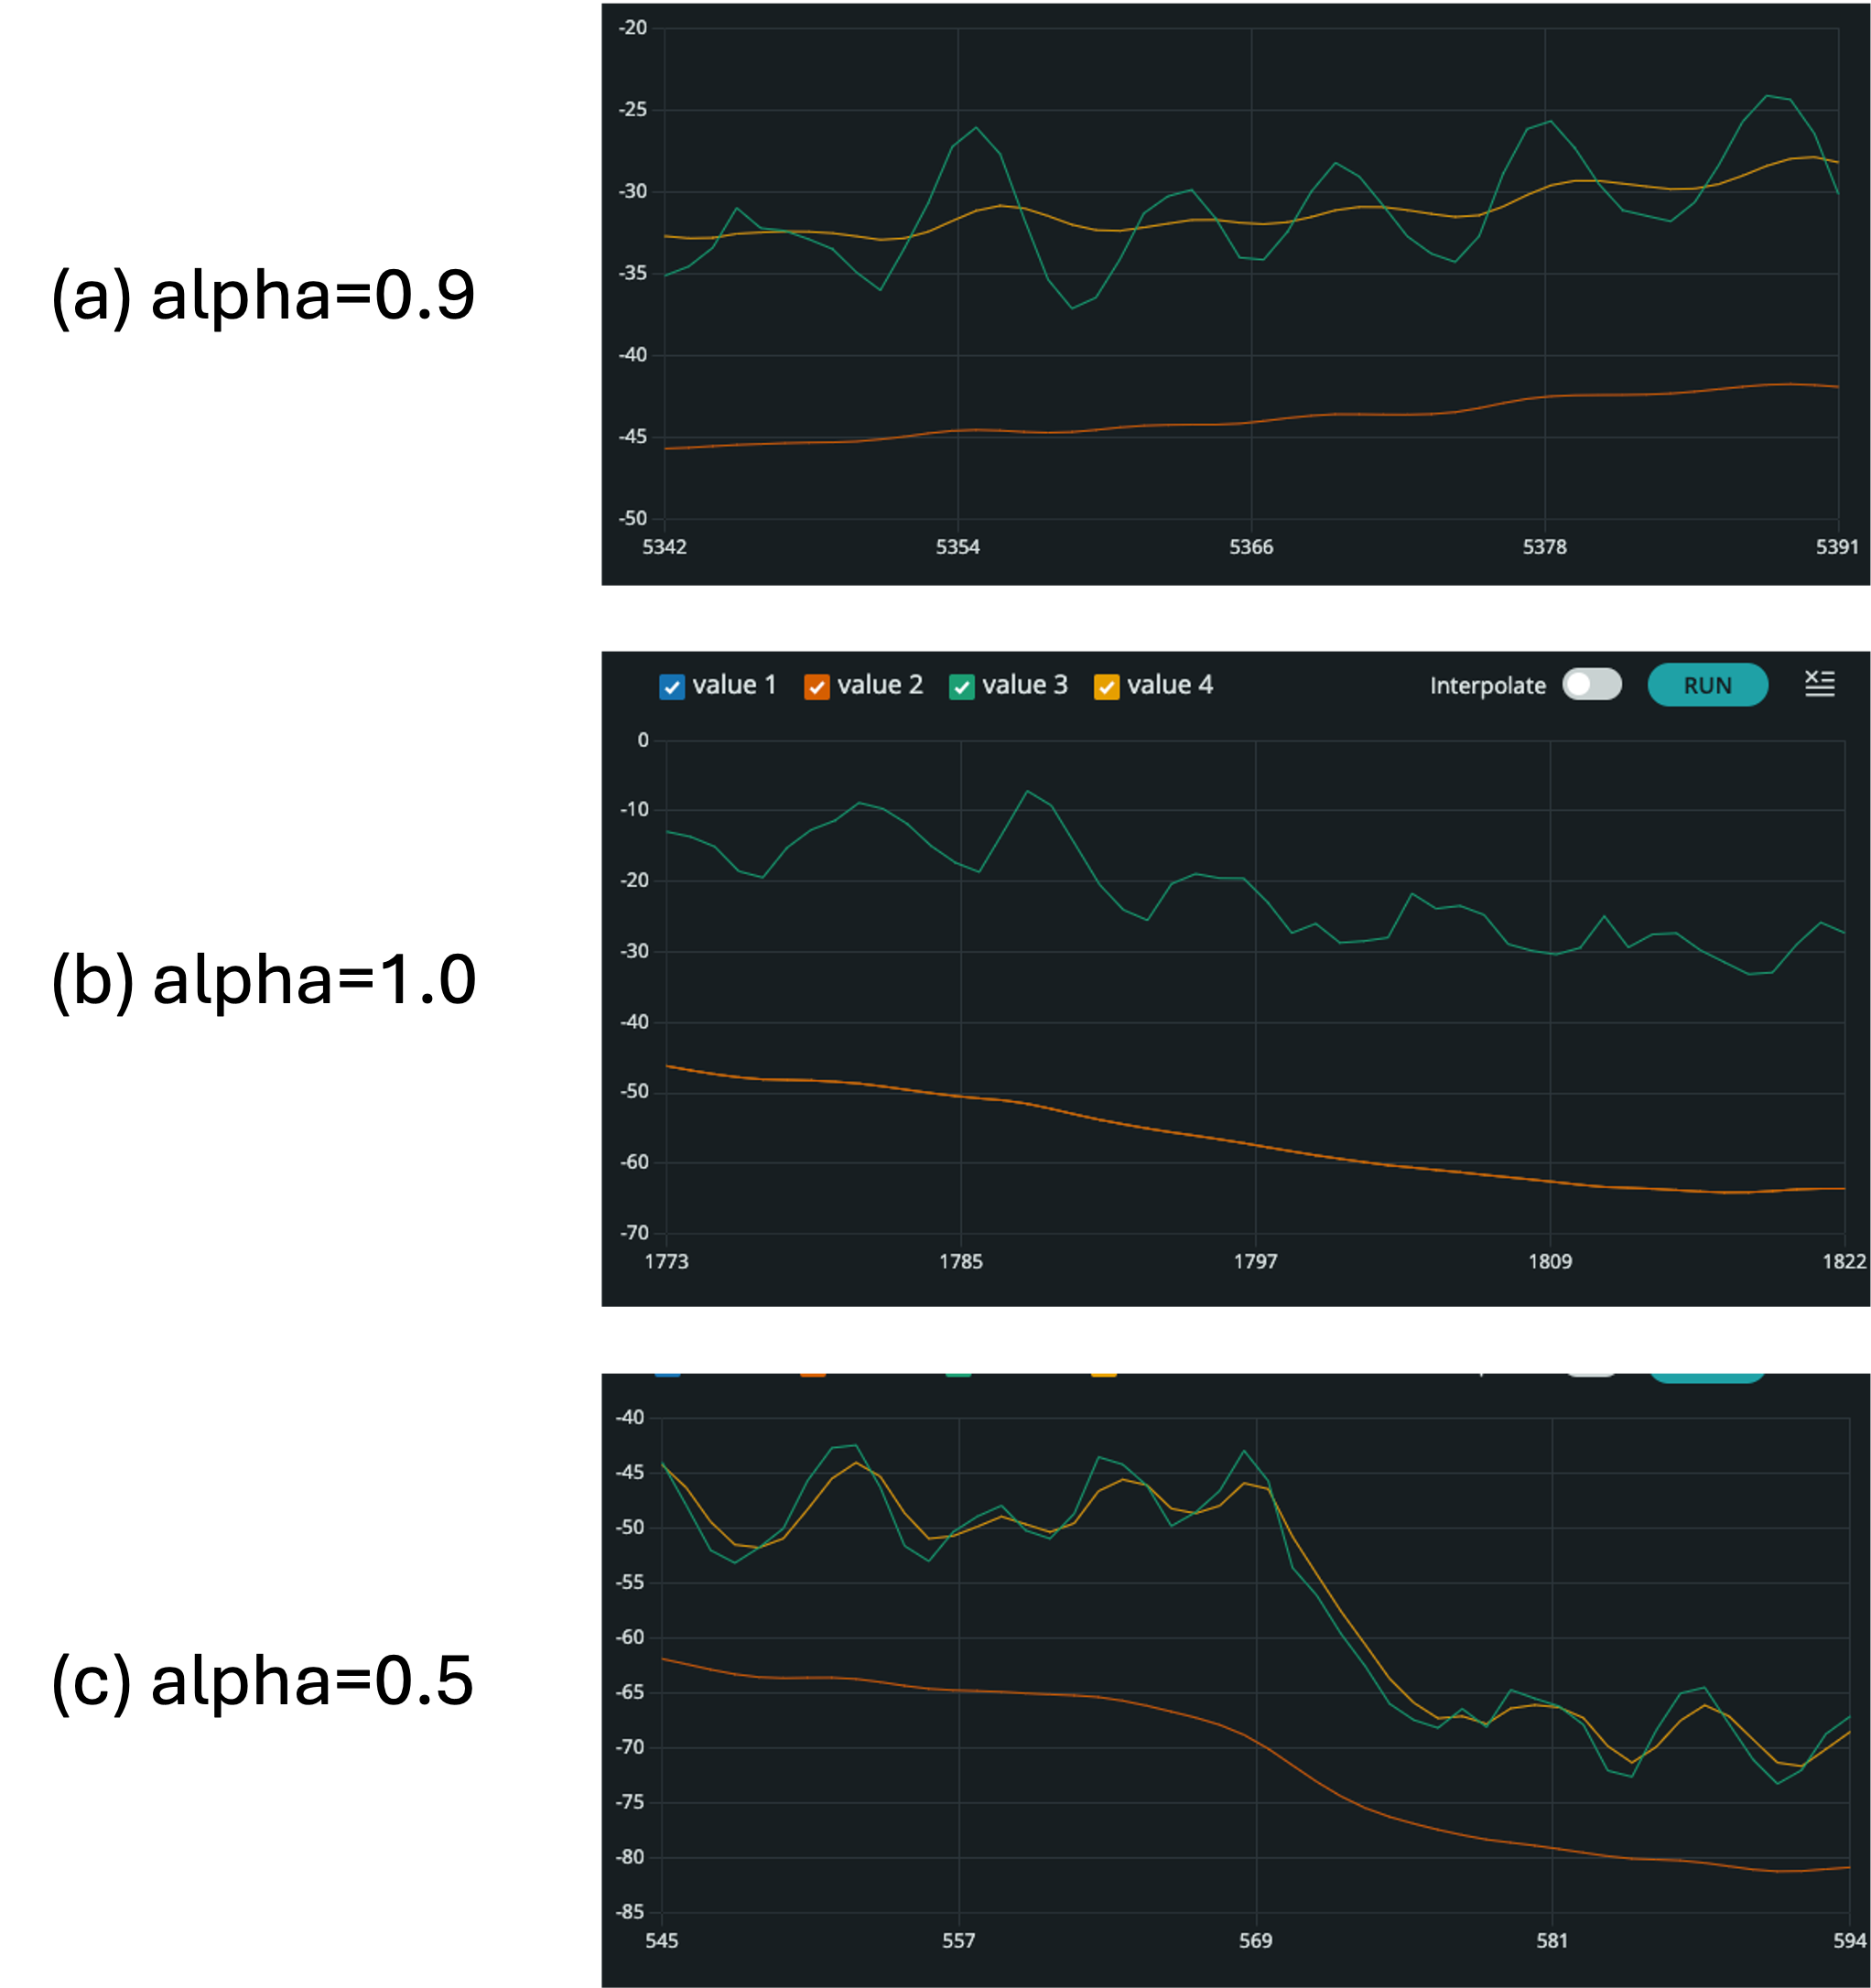
\includegraphics[width=0.7\textwidth]{figures/fig_threecurve.png}
\end{figure}
Description: The gyro-only curve is not noisy but has an offset from the groundtruth. The accelaration-only curve is noisy. The complementary filter resulting in low-noise result without global bias. Comparing the cases with different alpha values, for very small alpha, the complementary curve converges to the accelaration curve with large noise, while for large alpha, the complementary curve converges to the gyro-only curve with a bias. An intermediate level of alpha mixing factor can give a good result. 

\subsubsection*{2.4.4 Quaternion-Based Orientation Tracking Algorithm Comparison}
\begin{figure}[h!t]
    \centering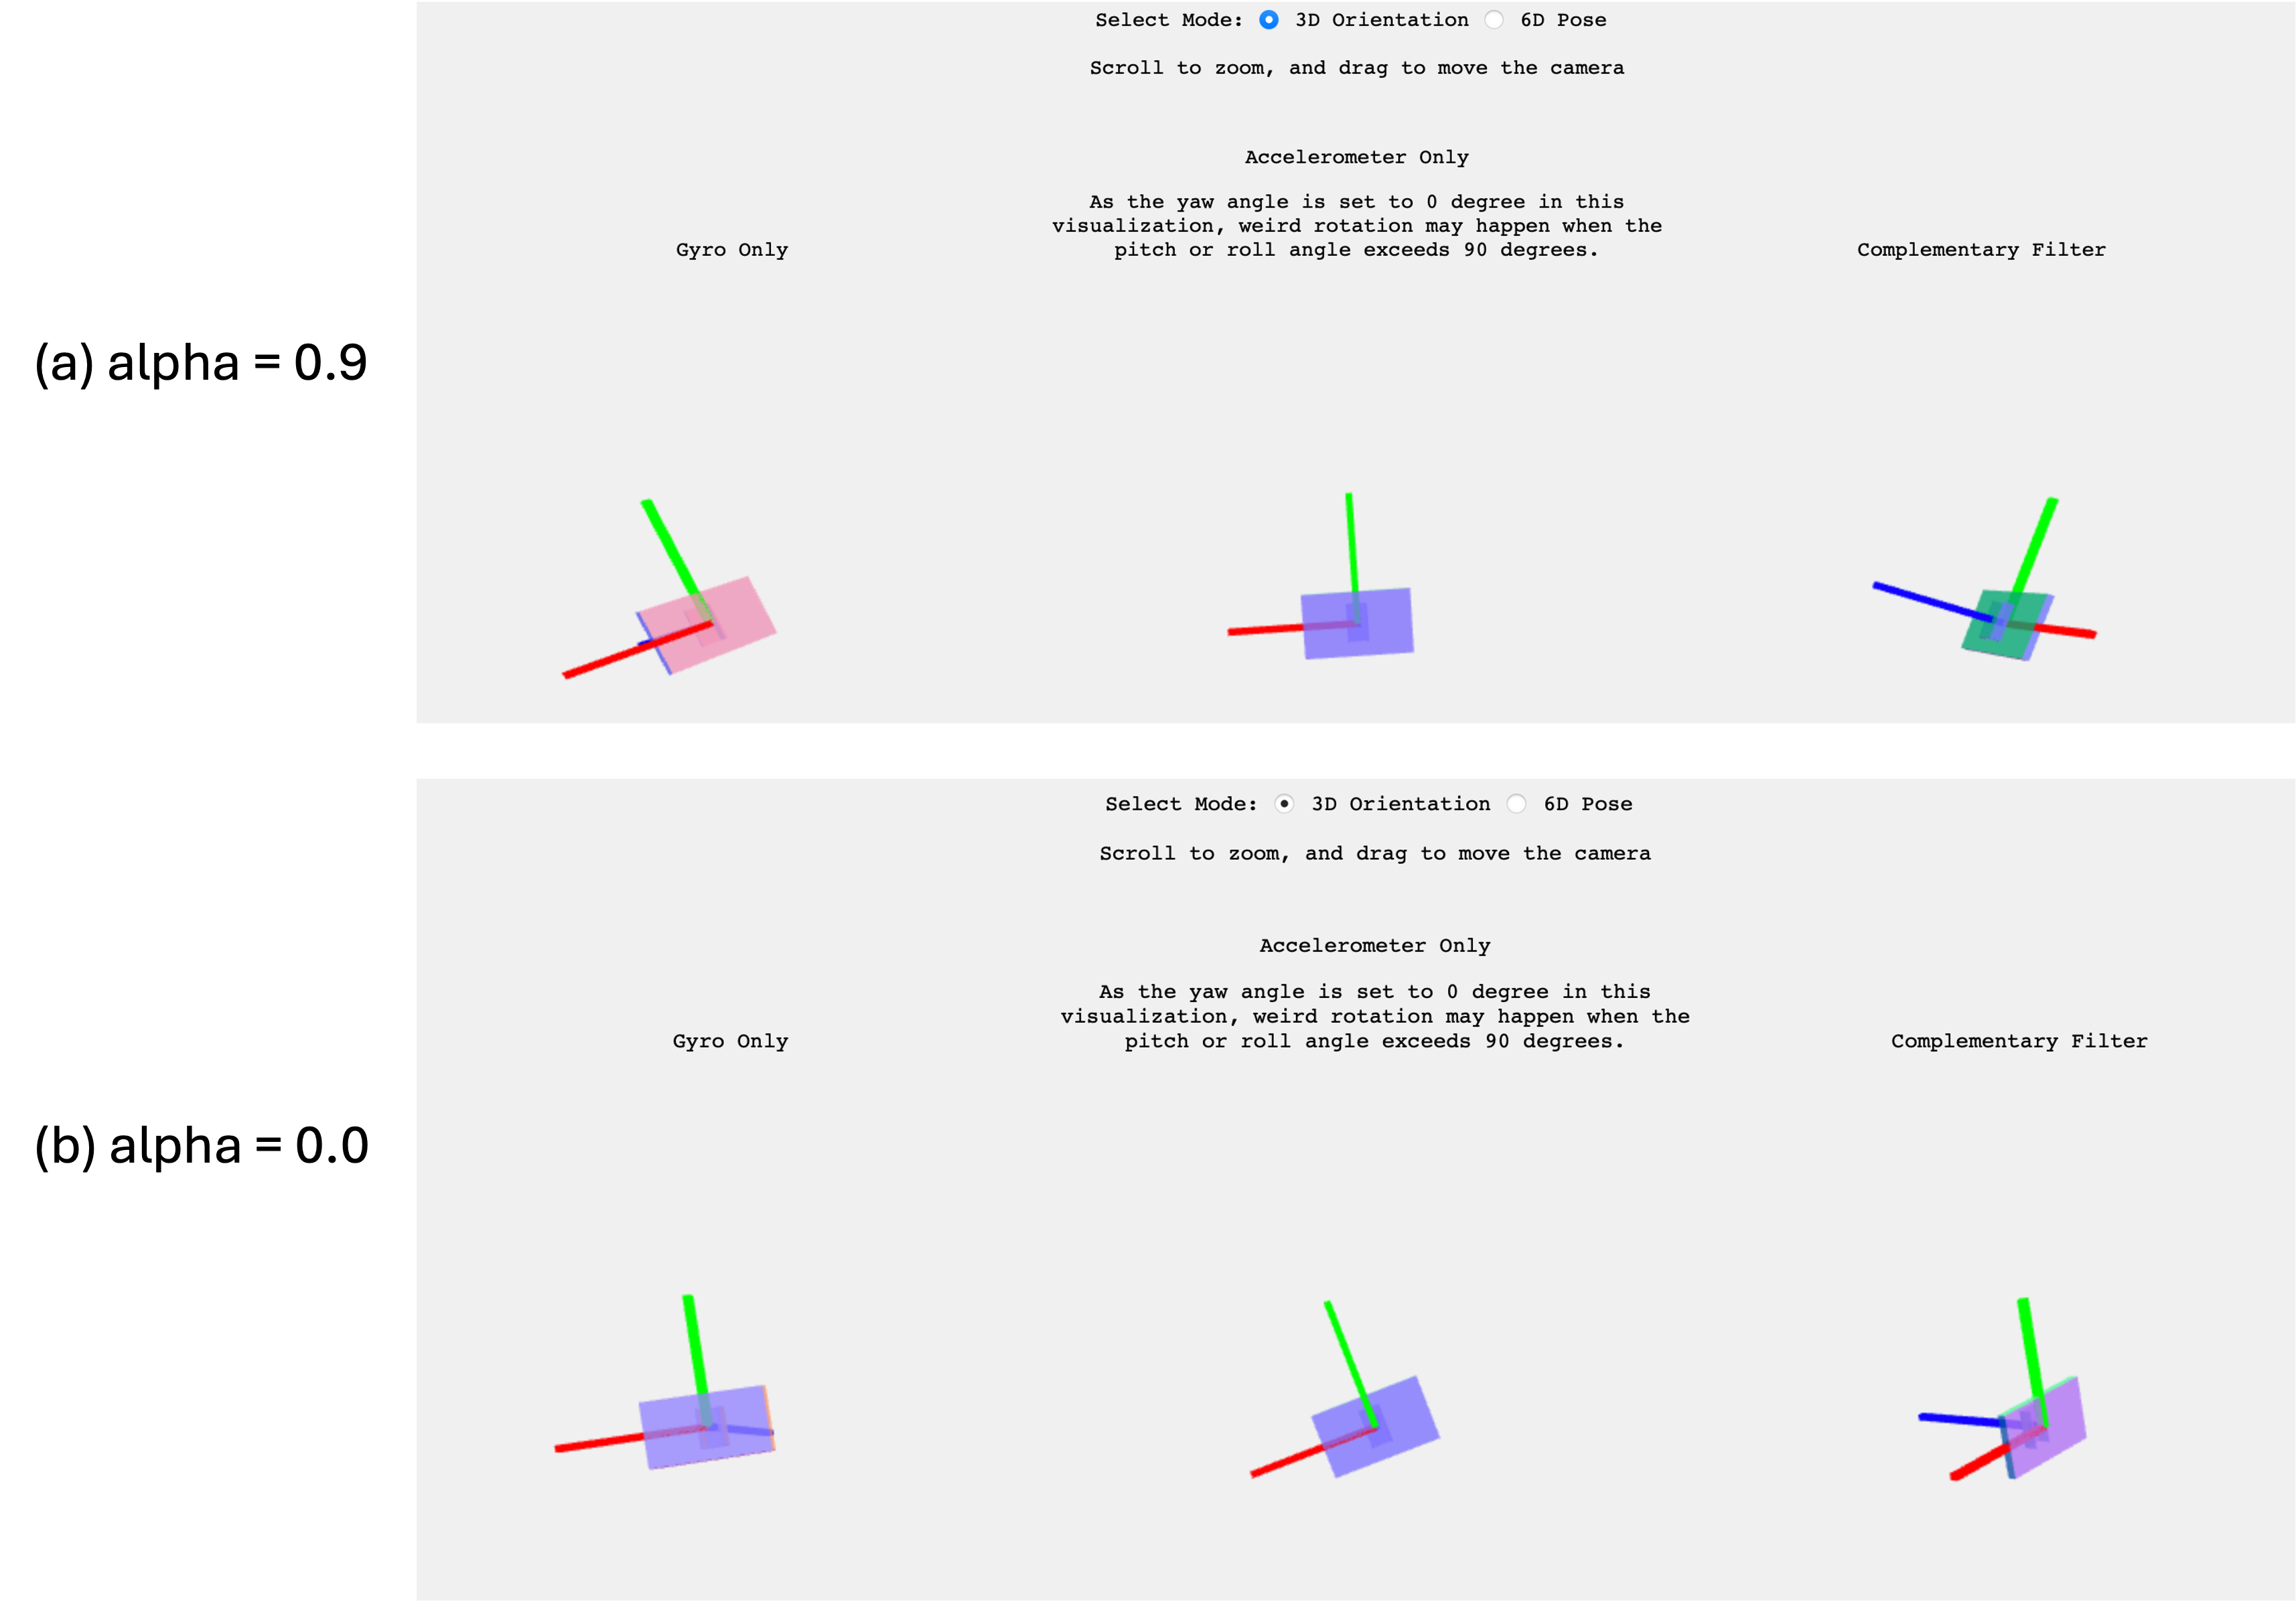
\includegraphics[width=0.7\textwidth]{figures/fig_quaternion1.png}
\end{figure}
Description: For the first case with $\alpha=0.9$, the comparison between the gyro-only motion and the motion given by the complementary filter shows that the they follow similar rotational motion. However there is a bias (offset) in between. For the second case (b) with $\alpha=0$, comparing acc-only motion with the motion given by the complementary filter shows that the z-axis follows the same orientation. However, due to the undefinable y-rotation in Euler angle, the accelerometer-only case cannot respond to y-rotation. On the other hand the complementary filter enables full rotation. Besides both cases show large noise. 

\subsubsection*{2.5.3 Head $\&$ Neck Model Discussion}
The actual motion parallex is actually quite obvious. For the case with head and neck model, when rotating head, the perspective changes a little bit as well, while it is not shown in the case without head and neck modelling. This helps to give a more realistic rendering scene! 


\end{document}